\chapter{Mapeo de Schwarz–Christoffel} \label{Schwarz–Christoffel }

\section{Introducción}\label{intro_SC}
El Teorema del mapeo de Riemann nos dice que cualquier simplemente conexa $\Omega$, estrictamente contenida en el plano complejo, podría ser transformada conformemente en el disco unitario abierto $D$ del plano complejo (Teorema \ref{TMR}), sin embargo este teorema de existencia no es constructivo, es decir, no se proporciona un método explicito para encontrar tal mapeo conforme.\\
En este capitulo se realiza un breve estudio del mapeo de Schwarz–Christoffel, este mapeo se define por una serie de puntos singulares en el borde del polígono y su correspondencia con puntos en el eje real del semiplano. La función de mapeo se construye a partir de una fracción algebraica que se integra en una función analítica específica. Además, el mapeo de Schwarz-Christoffel es una herramienta valiosa para la visualización y la solución de problemas en muchas áreas de la matemática, incluyendo la teoría de números, la teoría de sistemas dinámicos y la teoría de grupos. También es importante en la aplicación de las cálculo numérico y la teoría de la optimización en la solución de problemas en ingeniería y ciencias.

Además, el mapeo de Schwarz-Christoffel tiene propiedades únicas que lo hacen diferente de otras transformaciones conformes. Por ejemplo, es posible calcular el área y la longitud de curvas en un polígono a partir de su representación en un semiplano, lo que es útil para resolver problemas en geometría y teoría de curvas.

\section{Mapeo de Schwarz-Chrstoffel}
Consideremos una región simplemente conexa $\Omega$, cuya frontera sea un polígono de $n$ lados en el plano $w$ con vértices $w_1,w_2,\ldots,w_n$, en 1866 Hermann Amandus Schwarz e independientemente en 1867  Elwin Bruno Christoffel, publicaron una forma de mapear  el semiplano superior en  la región $\Omega$.
\begin{figure}[h!]
	\centering
	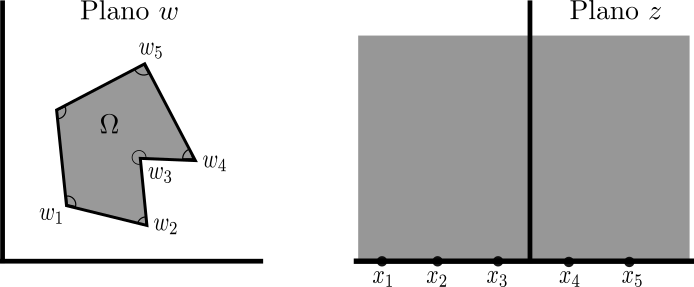
\includegraphics[width=0.7\linewidth]{img/sc}
	\caption{Transformacioón de Schwarz-Christoffel}
	\label{fig:sc}
\end{figure}
Suponga que cada $w_j$ se mapea en $x_j$, donde $x_j$ es un punto en el eje real.
La transformación que mapea el semiplano superior en   $\Omega$ esta definida  como 

\begin{equation}\label{dSC}
	\frac{dw}{dz}=C_1\prod_{j=1}^{n}(z-x_n)^{\frac{\phi_j}{\pi}-1}
\end{equation}
En forma integral
\begin{equation}\label{eSC}
	w=C_1\int \prod_{j=1}^{n}(z-x_n)^{\frac{\phi_j}{\pi}-1} dz +C_2
\end{equation}
donde $\phi_1,\ldots,\phi_n$ son los ángulos interiores de los vértices $w_j$.\\
La forma más sencilla de entender por qué funciona la fórmula es considerar una familia de incrementos infinitesimales $dz$ a lo largo del eje real en el plano $z$, y sus imágenes $dw$ en el plano $w$. La clave es explorar los argumentos (o fases) de estos cambios infinitesimales. Ahora la ecuación. (\ref{dSC}) nos dice que:
\begin{equation}\label{SC1}
	\mbox{Arg}(dw)=\mbox{Arg}(dz)+\mbox{Arg}(C_1)+\sum_{j=1}^{n}\left(\frac{\phi_j}{\pi}-1\right)\mbox{Arg}(z-x_j)
\end{equation}

A medida que $z$ se mueve a lo largo del eje real en la dirección positiva, cuando $z$ se encuentra estrictamente entre dos de los $x_j$,  todos los términos (\ref{SC1}) son constantes, de modo que $w$ se mueve en línea recta.
Esta es la razón por la que la imagen en el plano $w$ es poligonal. Ahora tenemos que ver qué sucede en las esquinas. Cuando $z$ pasa a través de $x_j$, todos los términos excepto aquellos que involucran a $x_j$ permanecen constantes, pero el factor $\mbox{Arg}(z-x_j)$ toma los siguientes valores
\[
	\mbox{Arg}(z-x_j)=\left\{\begin{array}{ccr}
		\pi &\mbox{si}&z<x_j\\
		0&\mbox{si}& z>x_j
	\end{array} \right.
\]
El término 
$$\left(\frac{\phi_j}{\pi}-1\right) \mbox{Arg}(z-x_j)$$



por lo tanto, salta del valor $\phi_j-1$ al valor $0$. La dirección en la que $w$ se está desplazando resulta ser un giro positivo (es decir, en sentido antihorario), por $\pi -\phi_j$. Un cambio de dirección por esta cantidad corresponde a la introducción de una esquina en el polígono con un ángulo interior $\phi_j$.\\

\iffalse Lo que esta discusión establece es que el eje real se mapea a la frontera de una región poligonal. Esto será suficiente para nuestros propósitos. Se puede ir más allá y establecer que el mapeo es uno a uno y, de hecho, toma el semiplano superior al interior de un polígono. Siempre podemos verificar este último punto calculando valores de muestra de mapeos particulares, como la imagen de $i$. \fi 



\subsection{Algunos comentarios sobre el punto en el infinito y los exponentes}
	Podemos asumir que uno de los puntos en el eje real, digamos $x_n$, está en el infinito, y que se elimina de la lista de puntos en la transformación. Para ver esto, escribimos, con $x_n <\infty$,
	
	$$C_1=\dfrac{C_1^{'}}{(-x_n)^{\frac{\phi_n}{\pi}-1}}$$
	$$\dfrac{\partial w}{\partial z}=C_1^{'}(z-x_1)^{\frac{\phi_1}{\pi}-1}(z-x_2)^{\frac{\phi_2}{\pi}-1}\cdots\left(\dfrac{x_n-z}{x_n}\right)^{\frac{\phi_n}{\pi}-1}$$
	
	Manteniendo  $C_1^{'}<\infty$ y tomando el límite $x_n\rightarrow \infty$ obtenemos 
	$$C_1=\dfrac{C_1^{'}}{(-x_n)^{\frac{\phi_n}{\pi}-1}}$$
	$$\dfrac{\partial w}{\partial z}=C_1^{'}(z-x_1)^{\frac{\phi_1}{\pi}-1}(z-x_2)^{\frac{\phi_2}{\pi}-1}\cdots(z-x_{n-1})^{\frac{\phi_{n-1}}{\pi}-1}$$
Recordemos que la suma de los ángulos exteriores de cualquier polígono cerrado es $2\pi$. Por lo tanto, podemos afirmar que
	$$\sum_{k=1}^{n}(\pi-\phi_k)=2\pi$$
	o bien, dividiendo entre $-\pi$
	$$\sum_{k=1}^{n}\left(\frac{\phi_k}{\pi}-1\right)=-2$$
	Por lo tanto, podemos afirmar que la suma de los exponentes en la fórmula \ref{eSC} es $-2$. Esto es una restricción que resultará útil en la relación entre la fórmula \ref{eSC} para un semiplano y el resultado correspondiente para un disco. También hay algo de libertad en la elección de los $x_n$. Tenga en cuenta que las constantes $C_1$ y $C_2$ simplemente ajustan el tamaño y la posición del polígono generado por el mapeo. Si establecemos $C_1 = 1 $ y $C_2 = 0$, creamos un polígono, digamos $P'$, que es similar al polígono deseado, digamos $P$, pero no tiene el tamaño correcto y no está en la ubicación correcta. Examinemos la libertad en los $x_j$ dentro de este esquema. Supondremos que $x_n = \infty$ aún no se ha realizado. En estas circunstancias, dado que los ángulos exteriores están fijos, todavía hay restricciones entre los $x_j$. Para que $P'$ sea similar a $P$, dado que los ángulos están fijos, requiere que los lados de $P'$ deban tener longitudes que están en una proporción constante común con los lados correspondientes de $P$. Esto implica $n - 3$ restricciones en los vértices, que a su vez están determinados por las $n$ variables $x_j$.\\
	Esto significa que antes de hacer que $x_n = \infty$, tres de los $x_j$ se pueden elegir a voluntad. Si hacemos que $x_n = \infty$, dos de los $x_j$ restantes se pueden elegir. Esta libertad también se puede entender en términos de los requisitos dentro del Teorema de mapeo de Riemann necesarios para hacer que el mapeo sea único: debemos especificar la imagen de un punto complejo  y una dirección para garantizar la unicidad.
	
	\subsection{Deducciones de las formulas \\de \SC}
	La discusión anterior aunque es informal nos da una idea de la transformación de \SC, a continuación se demuestra la formula de \SC para el semiplano superior
	\begin{teor}[Formula de \SC \; para el semiplano superior\index{Formula de \SC\; para el semiplano superior}]
		Sea $\Omega$ una región simplemente conexa cuya frontera sea un polígono con vértices $w_1,\ldots,w_n$ y ángulos interiores $\phi_1, \ldots,\phi_n $ en sentido antihorario. Sea $f$ cualquier mapeo conforme del semiplano superior $H$ a $\Omega$ con $f (\infty) = w_n$. Entonces
		\begin{equation}\label{SCSP}
			f(z)=C_1\int \prod_{j=1}^{n-1}(z-x_n)^{\frac{\phi_j}{\pi}-1} dz +C_2
		\end{equation}
		
		para algunas constantes $C_1$ y $C_2$, donde $w_j=f(x_j)$ para $j=1,2,\ldots,n-1$. 
		\proof Para simplificar, tratamos solo el caso donde todos los $x_j$ son finitos y el producto oscila entre los índices $1$ a $n$. Por el principio de reflexión de Schwarz,  el mapeo $f$ puede continuarse analíticamente en el semiplano inferior; la imagen continúa en el reflejo de $\Omega$ sobre uno de los lados del polígono. Al reflejar de nuevo sobre un lado del nuevo polígono, podemos regresar analíticamente al semiplano superior. Lo mismo se puede hacer para cualquier número par de reflexiones de $\Omega$, cada vez creando una nueva rama de $f$. La imagen de cada rama debe ser una copia trasladada y rotada de $\Omega$. Ahora, si $C_1$ y $C_2$ son constantes complejas, entonces
		$$\dfrac{(C_2+C_1f(z))''}{(C_2+Cf(z))'}=\dfrac{f''(z)}{f'(z)}$$
				Por lo tanto la función $\frac{f''(z)}{f'(z)}$ se puede definir por  continuación como una función univaluada en todas partes de la cerradura en el semiplano superior, excepto en los $z_j$ (donde las derivadas pueden no existir). Análogamente, considerando números impares de reflexiones, vemos que $\frac{f''(z)}{f'(z)}$ 	es univaluada y analítica en el semiplano inferior también.\\
		Afirmamos que dado $x_j$, se cumple que 
		$$f'(z)=(z-x_j)^{\frac{\phi_j}{\pi}-1}\psi(z)$$
		para una función analítica $\psi(z)$ en una vecindad de $x_j$. En efecto, puesto 	que la idea detrás de la transformación \SC  es que una transformación conforme $f$ pueda tener una derivada que se puede expresar 	como
		$$f'=\prod f_j$$
		 por el principio de reflexión de Schwarz, la función $f$ puede continuarse analíticamente a través del segmento $(x_j,x_{j+1})$.  En particular, $f'$ existe
		en este segmento, y vemos que $\mbox{arg} f'$ debe ser constante allí. Además, $\mbox{arg} f'$ debe experimentar un salto en $z = x_j$, a saber
		$$[\mbox{arg}f'(z)]_{x_j^{-}}^{x_j^{+}}=(1-\frac{\phi_j}{\pi})\pi=\beta_j\pi $$
		El ángulo $\beta_j\pi $ es el ángulo de giro en el $j$-ésimo vértice. Ahora identificamos una función $f_j$ que es analítica en el semiplano superior que  satisface $[\mbox{arg}f'(z)]_{x_j^{-}}^{x_j^{+}}=\beta_j\pi $, y  además tiene $\mbox{arg}f_j$ es constante en $\R$:
		$$f_j=(z-x_j)^{-\beta_j}$$
		tomando $f_j(z)>0$ si $z>x_j$ sobre $\R$ podemos formar
		$$f'(z)=K\prod_{j=1}^{n}f_j(z)$$
		donde $K$ es alguna constante. Lo anterior prueba la afirmación.\\
		Ya que $$f'(z)=(z-x_j)^{\frac{\phi_j}{\pi}-1}\psi(z)$$, entonces $\frac{f''(z)}{f'(z)}$  tiene un polo simple en $x_j$ con residuo $\frac{\phi_j}{\pi}-1$, y 
		$$\frac{f''(z)}{f'(z)}-\ds\sum_{j=1}^{n}\dfrac{\frac{\phi_j}{\pi}-1}{z-x_j}$$ es una función entera.Como $x_j<\infty$ para cada $j$, $f$ es analítica en $z=\infty$, y la expansión en series de Laurent implica que  $\frac{f''(z)}{f'(z)}\rightarrow0$ cuando $z\rightarrow\infty$, por el Teorema de Liouville se sigue que $$\frac{f''(z)}{f'(z)}-\ds\sum_{j=1}^{n}\dfrac{\frac{\phi_j}{\pi}-1}{z-x_j}$$
		es idénticamente cero. Expresando $\frac{f''}{f}$ como $(\ln (f'))'$ e integrando obtenemos la formula de \SC.\endproof
	\end{teor}
Existe una versión que mapea el disco unitario $D(0,1)$  en un polígono.
\begin{teor}[Formula de \SC \; para el disco] \index{Formula de \SC \; para el disco}
	Sea $\Omega$ una región simplemente conexa cuya frontera sea un polígono con vértices $w_1,\ldots,w_n$ y ángulos interiores $\phi_1, \ldots,\phi_n $ en sentido antihorario. Sea $f$ cualquier mapeo conforme del disco unitario $D(0,1)$ a $\Omega$. Entonces
	\begin{equation}\label{SCD}
		f(z)=A+C\int\prod_{k=1}^{n}\left(\dfrac{z}{x_k}-1\right)^{\frac{\phi_k}{\pi}-1}dz=\bar{C}\int\prod_{k=1}^{n}(p-p_j)^{\frac{\phi_k}{\pi}-1}dp+\bar{A}
	\end{equation}
	para algunas $A,C\in \C$, donde $w_k=f(x_k)$ para $k=1,2,\ldots,n$.
	\proof El mapeo 
	$$p(z)=\dfrac{z-i}{z+i}$$
	manda el semiplano superior al circulo unitario, la inversa de este mapeo resulta ser
	$$\dfrac{i(1+p)}{1-p}$$
	suponga que los $x_k$ son mapeados a puntos $p_k$ en el circulo unitario, entonces para cada $k$ tenemos
	$$z-x_k=\dfrac{i(p+1)}{1-p}-\dfrac{i(p_k+1)}{1-p_k}=\dfrac{2i(p-p_k)}{(1-p)(1-p_k)}$$
	y el Jacobiano de la transformación es 
	$$\dfrac{\partial z}{\partial p}=\dfrac{2i}{(1-p)^2}$$
	sustituyendo esto en la formula de \SC, usando el exponente de la formula 
	$$\sum_{k=1}^{n}\left(\frac{\phi_k}{\pi}-1\right)=-2$$
	y simplificando obtenemos la formula.\endproof
\end{teor}

	
	
\section{Ejemplos del uso de la formula de Schwarz-Chrstoffel para el semiplano}
	En esta sección se presentan una serie de ejemplos que nos permitirán tener una comprensión más clara de la fórmula \ref{eSC}, ahora consideraremos algunos ejemplos analíticos simples. No es difícil suponer que  la cuestión se complica un poco más cuando hay más de tres vértices, ya que entonces tenemos que resolver el problema de determinar los $x_j$ para todos menos tres de los valores de $j$. Así que consideraremos primero algunos casos con solo dos vértices, que se pueden hacer de manera analítica.  
	\subsection{Polígono con un vértice}
	Las formulas de \SC no son del todo explicitas, Debemos determinar los $x_j$ y las constantes afines $C_1$ y $C_2$ antes de poder aplicar la formula. Existe cierta flexibilidad en la selección de estos parámetros. Por el Teorema de mapeo de Riemann, podemos elegir cualquier tres puntos en $\R\setminus\{\infty\}$ para mapearlos a cualesquiera tres puntos de del polígono, siempre y cuando se mantenga su orden. En otras palabras, hay tres grados de libertad en el mapeo, lo que nos permite elegir tres  $x_j$ arbitrariamente. Por lo tanto, si $n \leq 3$, no hay problema de parámetros que debamos resolver y la fórmula \SC se vuelve explícita y en ocasiones sencilla de resolver.\\
	Cuando $n=1$, el polígono resulta ser una linea, con vértice  $w_1=\infty$ y $\phi_1=-\pi$, entonces $f(z)$ resulta ser de la forma
	$$f(z)=C_2+C_1z$$
	que permite el escalado, la rotación y la traslación. La fórmula del mapa del disco  \ref{SCD} nos da 
	$$f(z)=A+\dfrac{C}{z-z_1}$$
			Este es uno de los pocos resultados analíticos simples de la fórmula de Schwarz-Chrstoffel. 




	\subsection{La franja vertical semi-infinita.}
		Posiblemente el caso más simple es el de la franja vertical semi-infinita dada por:
		$$\Omega=\{ w\in \C : -a\leq \mbox{Re}(w)\leq a\; y \; \mbox{Im}(w)\geq 0  \}$$
		donde $a\in\R\setminus{0}$.\\
		En este caso tenemos:
		\[
			\begin{array}{lcr}
				w_1=-a;&&\phi_1=\frac{\pi}{2}\\
				w_2=a;&&\phi_2=\frac{\pi}{2}
			\end{array}
		\]
		y podemos simplemente tomar $x_1=-1$, $x_2=1$, entonces la forma diferencial de la ecuación de Schwarz-Chrstoffel nos da
		$$\frac{\partial w}{\partial z}=C_1(z-1)^{\frac{\frac{\pi}{2}}{\pi}-1}(z+1)^{\frac{\frac{\pi}{2}}{\pi}-1}=\dfrac{C_1}{\sqrt{z^2-1}}=\dfrac{A}{\sqrt{1-z^2}}$$
		donde el cambio de las constantes lo realizamos para que la ecuación nos sea más fácil de integrar, es decir,
		\[
			w=\int \frac{\partial w}{\partial x}dx=\int \dfrac{A}{\sqrt{1-z^2}}=B+A\sin^{-1}(z)
		\]
		Ahora las constantes $A$ y $B$ se pueden fijar mirando las ubicaciones de los vértices. Considerando el primer vértice, esto nos da:
		$$-a=B+A\sin^{-1}(-1)=B-\frac{A\pi}{2}$$
		El otro vértice nos da
		$$a=B+A\sin^{-1}(1)=B+\frac{A\pi}{2}$$
		resolviendo el sistema $2x2$ que se obtuvo, se tiene que $B=0$ y por consiguiente $$A=\frac{2a}{\pi}$$
		 así pues 
		\[
			\begin{array}{lcr}
				w=\frac{2a\sin^{-1}(z)}{\pi},&&z=\sin\left(\dfrac{\pi w}{2a}\right)
			\end{array}
		\]

	
		Consideremos cuando $a=1$, es decir
		\[
			\begin{array}{lcr}
				w=\frac{2\sin^{-1}(z)}{\pi},&&z=\sin\left(\dfrac{\pi w}{2}\right)
			\end{array}
		\]
		Podemos tener una mirada más detallada a lo que hace este mapeo usando las funciones que se construyeron en el capítulo 2.
		
		\begin{mmaCell}{Input}
  cartesianMap[func_, xrange_, yrange_, options___] := \\ParametricPlot[Evaluate[Through[\{Re, Im\}[func]]],\\xrange, yrange, options]
		\end{mmaCell}
	
	\newpage
		\begin{mmaCell}{Input}
  cartesianConformal[func_, xrange_, yrange_, options___] :=\\Show[GraphicsGrid[\{\{cartesianMap[x + I*y, xrange, yrange,\\options,DisplayFunction -> Identity],\\cartesianMap[W[x + I*y],xrange, yrange, options,\\DisplayFunction -> Identity]\}\}],\\DisplayFunction -> \$DisplayFunction]
		\end{mmaCell}
		
		
		\begin{mmaCell}{Input}
  w[z_] = (2*ArcSin[z])/Pi;\\cartesianConformal[w[x + I*y], \{x, -16, 16\}, \{y, 10^(-8), 16\},\\Mesh -> 50, LabelStyle -> Directive[Larger, Bold],\\PlotStyle -> White, MeshStyle -> Blue, Axes -> True,\\PlotPoints -> 200, PlotRange -> All]
		\end{mmaCell}
		\begin{mmaCell}[moregraphics={moreig={scale=0.7}}]{Output}
			\mmaFrac{ \mmaGraphics{28.png}}{}
		\end{mmaCell}
	
	\subsection{Triángulos}
		
	Los polígonos con tres vértices son los dominios más generales para los cuales los $x_j$ de la formula de  Schwarz-Christoffel pueden ser elegidos arbitrariamente, siempre y cuando permanezcan distintos y ordenados correctamente. Consideremos la siguiente imagen (los parámetros en la rutina de trazado, son con fines ilustrativos, no tienen un  significado en particular), donde asumimos que el punto $A$ está en el origen y $B$ está en $w =1+0i=1$. Los ángulos interiores en estos dos vértices son $\alpha$ y $\beta$ respectivamente.
	
\begin{mmaCell}{Input}
  Show[Graphics[\{\{LightBlue,Polygon[\{\{0,0\},\{1,0\},\{0.3,1\}\}]\},\\ \{PointSize[0.03], Point[\{0, 0\}]\},\{PointSize[0.03],\\Point[\{1, 0\}]\},\{PointSize[0.03], Point[\{0.3, 1\}]\}, \\Line[\{\{-1/2, 0\}, \{1.5, 0\}\}],Line[\{\{0, -1/2\}, \{0, 1.5\}\}],\\Text["A", \{0.1, -0.1\}], Text["B", \{1.1, -0.1\}],\\Text["C", \{0.3, 1.2\}],Text["[Alpha]", \{0.1, 0.1\}],\\Text["[Beta]", \{0.85, 0.1\}]\}]]
\end{mmaCell}
	
\begin{mmaCell}[moregraphics={moreig={scale=0.8}}]{Output}
	\mmaFrac{ \mmaGraphics{29.png}}{}
\end{mmaCell}

Lo que buscamos es construir de alguna manera un mapeo $w(z)$ tal que este triángulo sea la imagen del plano superior, con A situado en el origen z = 0, y B en z = 1. Aquí haremos uso del hecho de que C puede ser definido como $f(\infty)=C$, de modo que la fórmula \SC solo involucre dos términos:
$$\dfrac{\partial w}{\partial z}=A' z^{\frac{\alpha}{\pi}-1}(z-1)^{\frac{\beta}{\pi}-1}=Cz^{\frac{\alpha}{\pi}-1}(1-z)^{\frac{\beta}{\pi}-1}$$
integrando desde $\xi=0$ hasta $\xi=z$
$$w=C\int_{0}^{z}\xi^{\frac{\alpha}{\pi}-1}(1-\xi)^{\frac{\beta}{\pi}-1}d\xi+B$$
Ahora, cuando $z = 0$, también queremos que $w = 0$, por lo que ponemos $B = 0$. Además, dado que $w = 1$ cuando $z = 1$, debemos elegir a $C$ tal que se cumpla:
$$1=C\int_{0}^{1}\xi^{\frac{\alpha}{\pi}-1}(1-\xi)^{\frac{\beta}{\pi}-1}d\xi+B$$
Utilizamos a continuación la función \textbf{Integrate} de Mathematica
\begin{mmaCell}{Input}
	 Integrate[\mmaSup{\mmaFnc{\(\pmb{\xi}\)}}{\mmaFrac{\mmaUnd{\(\pmb{\alpha}\)}}{\mmaDef{\(\pmb{\pi}\)}}-1}\mmaSup{(1-\mmaFnc{\(\pmb{\xi}\)})}{\mmaFrac{\mmaUnd{\(\pmb{\beta}\)}}{\mmaDef{\(\pmb{\pi}\)}}-1},\{\mmaFnc{\(\pmb{\xi}\)},0,1\},Assumptions\(\pmb{\to}\)\{\mmaUnd{\(\pmb{\alpha}\)}>0,\mmaUnd{\(\pmb{\beta}\)}>0\}]
\end{mmaCell}
obtenemos
$$\dfrac{\Gamma\left(\frac{\alpha}{\pi}\right)\Gamma\left(\frac{\beta}{\pi}\right)}{\Gamma\left(\frac{\alpha+\beta}{\pi}\right)}$$
por lo tanto 
$$C=\dfrac{\Gamma\left(\frac{\alpha+\beta}{\pi}\right)}{\Gamma\left(\frac{\alpha}{\pi}\right)\Gamma\left(\frac{\beta}{\pi}\right)}$$
por lo tanto el mapeo viene dado por 
\begin{equation}
	w=\dfrac{\Gamma\left(\frac{\alpha+\beta}{\pi}\right)}{\Gamma\left(\frac{\alpha}{\pi}\right)\Gamma\left(\frac{\beta}{\pi}\right)}\int_{0}^{z}\xi^{\frac{\alpha}{\pi}-1}(1-\xi)^{\frac{\beta}{\pi}-1}d\xi
\end{equation}
Recordemos que  $$\int_{0}^{z}\xi^{a-1}(1-\xi)^{b-1}d\xi = \beta_z(a,b)$$
donde $\beta_z(a,b)$ es la función beta incompleta, en \textbf{Mathematica} esta función especial puede usarse utilizando el comando \textbf{Beta[z,a,b]}.\\
Por otro lado, la función Beta se puede expresar en términos de la función Gamma
\[
	{\displaystyle {\begin{aligned}\Gamma (x)\Gamma (y)&=\int _{u=0}^{\infty }u^{x-1}e^{-u}du\int _{v=0}^{\infty }v^{y-1}e^{-v}dv\\&=\int _{v=0}^{\infty }\int _{u=0}^{\infty }u^{x-1}v^{y-1}e^{-u-v}dudv\end{aligned}}}
\]
haciendo el cambio $u=zt$ y $v=z(1-t)$

\[
	\displaystyle {\begin{aligned}\Gamma (x)\Gamma (y)&=\int _{z=0}^{\infty }\int _{t=0}^{1}e^{-z}(zt)^{x-1}(z(1-t))^{y-1}zdtdz\\&=\int _{z=0}^{\infty }e^{-z}z^{x+y-1}dz\int _{t=0}^{1}t^{x-1}(1-t)^{y-1}dt\\&=\Gamma (x+y)\beta (x,y)\end{aligned}}
\]
despejando obtenemos
\[
	{\displaystyle \beta (x,y)={\frac {\Gamma (x)\Gamma (y)}{\Gamma (x+y)}}}
\]
En \textbf{Mathematica} la función beta se puede usar usando el comando \textbf{Beta[a,b]}
así 
$$w=\dfrac{\beta_z\left(\frac{\alpha}{\pi},\frac{\beta}{\pi}\right)}{\beta\left(\frac{\alpha}{\pi},\frac{\beta}{\pi}\right)}$$
teniendo esto en cuenta escribimos la expresión para $w$ en \textbf{Mathematica}
\begin{mmaCell}{Input}
    w[z_,\(\alpha\)_,\(\beta\)_]:=\mmaFrac{Beta[z,\(\alpha\),\(\beta\)]}{Beta[\(\alpha\),\(\beta\)]}
\end{mmaCell}
En \textbf{Mathematica} contamos con una función que simplifica a la expresión anterior, esta es la función \textbf{BetaRegularized}, esta función da la función beta incompleta regularizada $I_z(a,b)$  y para casos no singulares se verifica 
$$I_z(a,b)=\dfrac{\beta(z,a,b)}{\beta(a,b)}$$
Ya con esto podemos reescribir a $w$ en Wolfram de la siguiente manera
\begin{mmaCell}{Input}
	 w[z_,\(\alpha\)_,\(\beta\)_]:=BetaRegularized[z,\(\alpha\),\(\beta\)]
\end{mmaCell}
Verifiquemos esta formula para el caso donde el triángulo es equilátero, con $\alpha=\beta=\frac{\pi}{3}$
\begin{mmaCell}{Input}
  ClearAll[z, w, k]\\w[z_] = BetaRegularized[z, 1/3, 1/3]\\cartesianConformal[w[x + I*y],\{x, -8, 8\}, \{y, 10^(-12), 8\},\\Mesh -> 60, LabelStyle -> Directive[Larger, Bold],\\PlotStyle -> AbsoluteThickness[0.01], MeshStyle -> Blue,\\Axes -> True,PlotPoints -> 1000, PlotRange -> All]
\end{mmaCell}
\begin{mmaCell}[moregraphics={moreig={scale=0.8}}]{Output}
	\mmaFrac{ \mmaGraphics{30.png}}{}
\end{mmaCell}
\subsection{Rectángulos y funciones elípticas}
Si $n = 4$, los $x_j$ de la formula de \SC no los podemos tomar a nuestra elección. En el caso general, no existe una manera analítica respecto al grado de libertad en los $x_j$. Sin embargo, en el caso importante cuando la región es el interior de un rectángulo, podemos usar la  simetría para hallar una solución explícita.
\begin{figure}[h!]
	\centering
	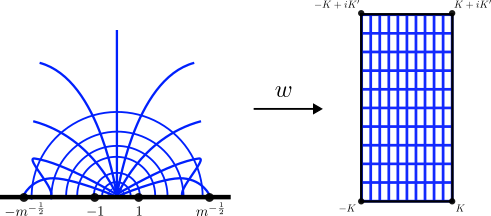
\includegraphics[width=0.72\linewidth]{img/SCR}
	\caption{Mapeo del semiplano superior a un rectángulo}
	\label{fig:scr}
\end{figure}
Rotamos y trasladamos el rectángulo para que sus vértices sean $w_1=-K+iK$, $w_2=-K$, $w_3=K$ y $w_4=K+iK$. Por simetría elegimos los $x_j$ como $z_1 = -m$, 
$z_2 = -1$, $z_3 = 1$ y $z_4 = m$,  donde $m$ es un parámetro que representa el grado de libertad en los $x_j$. La imagen del infinito resulta ser  el punto $iK'$, y la imagen de $0$ es $0$. La función puede escribirse como una integral elíptica de primera clase:
\[
	\begin{array}{ccl}
		w&=&C_1\ds\int_{}^{z}\prod_{j=1}^{4}(t-x_j)^{-\frac{1}{2}}dt+C_2\\
		&=&-C_1\ds\int_{}^{z}\dfrac{dt}{\sqrt{(m^{2}-t^2)(1-t^2)}}
	\end{array}
\]
resulta más conveniente hacer el cambio de variable $a=m^{-1}$, $C_1'=-C_1$, entonces 
\[
	\begin{array}{ccl}
		w&=&C_1'\ds\int_{}^{z}\dfrac{dt}{\sqrt{(1-a^2t^2)(1-t^2)}}\\
		=&=&C_1'\ds\int_{}^{\sin^{-1}(z)}\dfrac{d\theta}{\sqrt{1-a^2\sin^2(\theta)}}
	\end{array}
\]
Esta integral se conoce como integral elíptica incompleta de primera clase. \textbf{Mathematica} cuenta con una serie de funciones ya definidas para las integrales elípticas, en este ejemplo la función que usaremos seria \textbf{EllipticF[$\phi$, m]} la cual nos da la integral elíptica de primer orden $F(\phi|m)$.\\
Ingresando esta ultima integral en \textbf{Mathematica}
\begin{mmaCell}{Input}
  Integrate[1/(Sqrt[1 - a*Sin[z]^2]), \{z, 0, ArcSin[z]\}]
\end{mmaCell}
obtenemos el siguiente resultado\\
\fbox{$F\left(\left.\sin ^{-1}(z)\right|a\right)\text{ if }0<\R\left(\sin ^{-1}(z)\right)\leq \frac{\pi }{2}\lor -\frac{\pi }{2}\leq \R\left(\sin ^{-1}(z)\right)<0$}
Para conocer más a detalle estas funciones en \textbf{Mathematica} vea \cite{Elliptic}.\\
Para simplificar este tomemos $c_1'=1$ y $m=2$, entonces $a=\frac{1}{2}$
\begin{mmaCell}{Input}
	 ClearAll[z, w];\\w[z_] = EllipticF[ArcSin[z], 0.5^2];\\cartesianConformal[w[x + I*y], {x, -8, 8}, \{y, 10^(-12), 8\},\\Mesh -> 60, LabelStyle -> Directive[Larger, Bold],\\PlotStyle -> AbsoluteThickness[0.01], MeshStyle -> Blue,\\Axes -> True, PlotPoints -> 1000, PlotRange -> All]
\end{mmaCell}
\begin{mmaCell}[moregraphics={moreig={scale=0.8}}]{Output}
	\mmaFrac{ \mmaGraphics{31.png}}{}
\end{mmaCell}
\section{Ejemplos del uso de la formula de Schwarz-Christoffel para el disco unitario}
En este caso, podemos hacer uso de la simetría para considerar puntos $p_j$ que estén espaciados uniformemente alrededor del círculo unitario, incluso podemos tomar los puntos $_j$ de tal forma que sean las raíces $n$-ésimas de la unidad de
$$p_j=\omega_n^j$$
$$\omega_n^{\frac{2\pi i}{n}}$$
El producto $(p-p_1)\cdots (p-p_n)$ se simplifica a $p^n-1$. Tenemos por objetivo un $n$-ágono regular, los ángulos interiores para un $n$-ágono son todos iguales y están dados por:
$$\phi_k=\pi\left(1-\dfrac{2}{n}\right)$$
y los exponentes son todos iguales a $-\frac{2}{n}$. Por lo tanto, el mapeo deseado es de la forma 
\begin{equation}
	w=\bar{A}\ds\int \dfrac{dp}{(p^n-1)^{\frac{n}{2}}}+B
\end{equation} 
Considerando los límites desde $p=0$ hasta $p=z$ y tomando $A=1$ obtendremos resultados más claros
\begin{equation}\label{SCn}
	w=\ds\int_{0}^{z}\dfrac{dp}{(1-p^n)^{\frac{n}{2}}}
\end{equation}
\subsection{El hexágono}
Se obtiene un hexágono regular al establecer $n = 6$ en la ecuación (\ref{SCn}).
\begin{mmaCell}{Input}
	 Integrate[1/(1 - p^6)^(1/3), {p, 0, z}]
\end{mmaCell} 
\vspace{-0.5 cm}donde obtenemos\\
\fbox{$z \, _2F_1\left(\frac{1}{6},\frac{1}{3};\frac{7}{6};z^6\right)\text{ if }-1<\text{Re} z\leq 1\lor z\notin \mathbb{R}$}\\
donde $_2F_1$ es la función hipergeométrica, en \textbf{Mathematica} esta función se escribe \textbf{ Hypergeometric2F1[a,b,c,z] }. Para más detalles puede consultar \cite{Hypergeometric2F1}.\\
Para comprobar qué está haciendo esta función usamos la función \textbf{polarConformal} que construimos anteriormente
\begin{mmaCell}{Input}
	 ClearAll[f, z]\\f[z_] = z Hypergeometric2F1[1/6, 1/3, 7/6, z^6]\\polarConformal[f[r Exp[I t]], {r, 0, 1},\\\{t, 0, 2*Pi\},Mesh -> \{50, 50\}, PlotRange -> All,\\LabelStyle -> Directive[Larger, Bold], PlotStyle -> White,\\MeshStyle -> Blue, Axes -> True]
\end{mmaCell}
\begin{mmaCell}[moregraphics={moreig={scale=0.8}}]{Output}
	\mmaFrac{ \mmaGraphics{32.png}}{}
\end{mmaCell}

\subsection{El $n$-ágono regular}
Con las consideraciones hechas previamente ahora nos resulta sencillo tratar el $n$-ágono regular
\begin{mmaCell}{Input}
	 nAgon[z_, n_] = Integrate[1/(1 - p^n)^(2/n), \{p, 0, z\},\\Assumptions -> n > 0]]
\end{mmaCell} 
obtenemos la siguiente expresión en términos de la función hipergeométrica
$$z \, _2F_1\left(\frac{1}{n},\frac{2}{n};1+\frac{1}{n};z^n\right)$$
Ahora, solo basta cambiar el parámetro $n$.\\
Las siguientes imágenes se generaron usando $n=3,4,5,10$ en el código
\begin{mmaCell}{Input}
	 ClearAll[f, z]\\polarConformal[nAgon[r Exp[I t], n], \{r, 0, 1\},\{t, 0, 2*Pi\},\\Mesh -> \{100, 100\}, PlotRange -> All,\\LabelStyle -> Directive[Larger, Bold],PlotStyle -> White,\\MeshStyle -> Blue, Axes -> True]
\end{mmaCell}
las imágenes obtenidas las podemos ver en la figura \ref{fig:Mapeo del círculo unitario al n-ágono}. \newpage
\begin{figure}[htbp]
	\centering
	\begin{subfigure}{0.45\textwidth}
		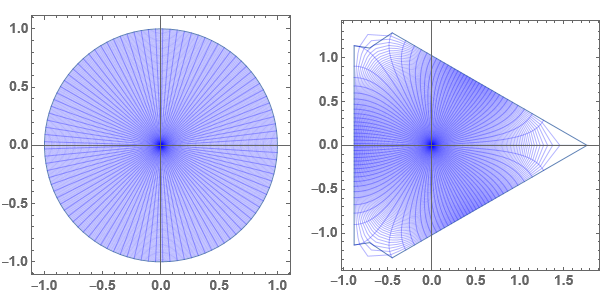
\includegraphics[width=\linewidth]{33.png}
		\caption{Mapeo del círculo unitario al triángulo.}
		\label{fig:Mapeo del círculo unitario al triángulo.}
	\end{subfigure}
	\begin{subfigure}{0.45\textwidth}
		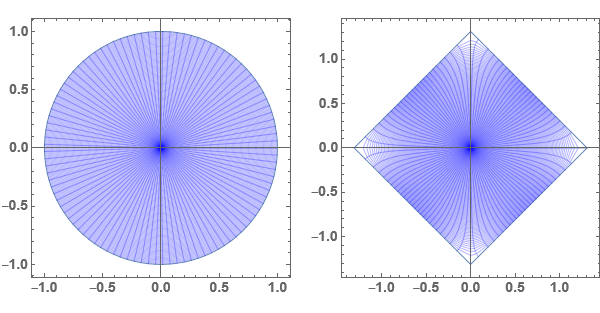
\includegraphics[width=\linewidth]{34.png}
		\caption{Mapeo del círculo unitario al cuadrado.}
		\label{fig:Mapeo del círculo unitario al cuadrado}
	\end{subfigure}
	
	\begin{subfigure}{0.45\textwidth}
		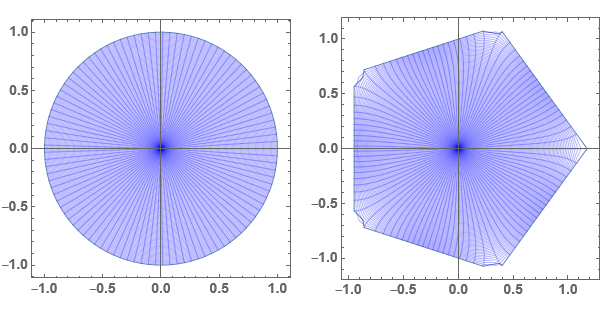
\includegraphics[width=\linewidth]{35.png}
		\caption{Mapeo del círculo unitario al pentágono.}
		\label{fig:Mapeo del círculo unitario al pentágono}
	\end{subfigure}
	\begin{subfigure}{0.45\textwidth}
		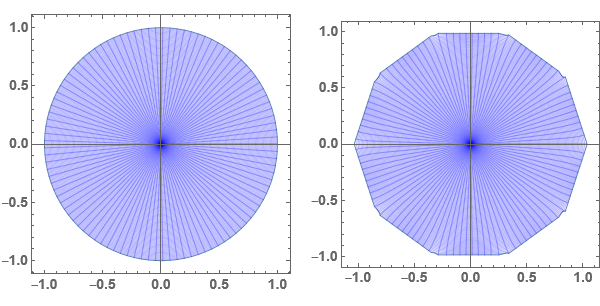
\includegraphics[width=\linewidth]{36.png}
		\caption{Mapeo del círculo unitario al decágono.}
		\label{fig:Mapeo del círculo unitario al decágono}
	\end{subfigure}
	\caption{Mapeo del círculo unitario al n-ágono}
	\label{fig:Mapeo del círculo unitario al n-ágono}
\end{figure}

\begin{comment}
	\section{Formula de Schwarz-Christoffel para superficies de Riemann}
	La formula de \SC vimos que es derivada del supuesto que los se satisface
	$$\sum_{k=1}^{n}\left(\frac{\phi_k}{\pi}-1\right)=-2$$
	En otras palabras, los giros exteriores suman $2\pi$. La fórmula se puede extender, sin embargo, para encontrar el mapeo $f$ del semiplano superior en el caso donde
	$$\sum_{k=1}^{n}\left(\frac{\phi_k}{\pi}-1\right)=-2(b+1)$$
	donde $b\in \N$. Tal región ya no esta en el plano, esta región es una superficie de Riemann.
	con $b + 1$ capas. Las capas se unen en los puntos $\sigma_1, \ldots , \sigma_b$, que son
	puntos de ramificación de la función multivaluada $w^{-1}$ al semiplano superior. Este argumento implica que $w'$ debe de tener a lo más $b$ ceros en el semiplano superior. Estos puntos $s_1,\ldots,s_b$ son preimágenes de los puntos de ramificación. Por lo que introducimos los factores $(z-s_k)$ a $w'$. Para evitar que estos afecten al $\mbox{arg }w'$ en el eje real, debemos multiplicar por $(z-\bar{s_k})$. El mapeo del semiplano superior a una superficie de Riemann es por tanto
	\begin{equation}
		w=A+C\ds\int_{}^{z}\prod_{k=1}^{b}(\zeta-s_k)(\zeta-\bar{s_k})\prod_{k=1}^{n-1}(\zeta-x_k)^{\frac{\alpha}{\pi}-1}d\zeta
	\end{equation}
	Las $2b$ incógnitas reales adicionales (las raíces de $w'$) se determinan requiriendo
	que $w (s_k) = \sigma_k$ para $k = 1, \ldots , b$. Estas incógnitas se pueden transformar para incorporar implícitamente sus limitaciones naturales. 
\end{comment}

\printbibliography[heading=bibintoc]



 